\documentclass{szte-thesis}

\title{Minta szakdolgozat címe}
\author{Kiss Péter}
%\neptun{ABC123}

% bsc / msc / tdk
\setdegree{bsc}

% titkos-e a szakdolgozat
\setconfidential{false}

\faculty{Természettudományi és Informatikai Kar}
\institute{Informatika Intézet}

% 1. témavezető tanszéke (rövid forma, pl. Szoftverfejlesztés)
\department{Szoftverfejlesztés}

\program{Programtervező informatikus}
%\specialization{Szoftverfejlesztő}

% 1. témavezető
\supervisor{Dr. Nagy Béla}
\supervisortitle{egyetemi docens}
% opcionálisan külön is megadhatod (ha nem a \department értéke kellene):
% \supervisordepartment{Szoftverfejlesztés}

% 2. témavezető
%\secondsupervisor{Dr. Kovács Anna}
%\secondsupervisortitle{adjunktus}
%\secondsupervisordepartment{Alkalmazott Informatika}

% Konzulens
\consultant{Nagy János}
\consultantworkplace{FrontEndArt kft.}
\consultantposition{Lead developer}

\city{Szeged}
\thesisyear{2025}
\thesislogo{img/szte\_logo}

\addbibresource{references.bib}

% Kapcsolók
\setboolean{showfigures}{true}
\setboolean{showtables}{true}
\setboolean{showcode}{true}
\setboolean{showtodos}{true}

\begin{document}
	
	\makecover
	
	\tableofcontents
	

\chapter{Metaadatok}

Ebben a fejezetben a \texttt{szte-thesis} osztályban használt metaadat-parancsokat mutatjuk be.  
Ezeket tipikusan a \texttt{main.tex} elején adjuk meg, még a \verb|\begin{document}| előtt.  

\section{Alap adatok: cím, szerző, Neptun-kód}

A dolgozat legfontosabb adatai:

\begin{itemize}
  \item \verb|\title{...}| -- a dolgozat címe,
  \item \verb|\author{...}| -- a hallgató neve,
  \item \verb|\neptun{...}| -- a Neptun-kód (ha használni szeretnénk).
\end{itemize}

\noindent
A \texttt{code/ch01-metaadatok-main.tex} fájl egy minimális példa ezekre.  
A kódot a következő módon importáljuk, kikapcsolható kódként:

\inputcode[Minden kötelező metaadat megadása]{TeX}{code/ch01-metaadatok-main.tex}

\section{Fokozat és titkosság}

A dolgozat típusát a \verb|\setdegree| paranccsal adjuk meg:

\begin{itemize}
  \item \verb|\setdegree{bsc}| -- BSc szakdolgozat,
  \item \verb|\setdegree{msc}| -- MSc diplomamunka,
  \item \verb|\setdegree{tdk}| -- TDK dolgozat.
\end{itemize}

\noindent
A titkosságot a \verb|\setconfidential{true}| vagy \verb|\setconfidential{false}| parancs állítja be.  
Ha a szakdolgozat titkosított, akkor az érték \verb|true|, ellenkező esetben \verb|false|.  
A hozzá tartozó példa a \texttt{code/ch01-degree-confidential.tex} fájlban található:

\inputcode[Fokozat és titkosság beállítása]{TeX}{code/ch01-degree-confidential.tex}

\section{Szak, szakirány, tanszék}

A szakhoz és a szakirányhoz tartozó metaadatokat az alábbi parancsokkal adjuk meg:

\begin{itemize}
  \item \verb|\program{...}| -- a szak neve,
  \item \verb|\specialization{...}| -- szakirány,
  \item \verb|\department{...}| -- az első témavezető tanszéke.
\end{itemize}

\noindent
Példa ezek használatára:

\inputcode[Szak, szakirány és tanszék megadása]{TeX}{code/ch01-program-department.tex}

\section{Témavezető és egyéb szereplők}

Az első témavezető, a második témavezető és a konzulens adatai a következő parancsokkal állíthatók be:

\begin{itemize}
  \item \verb|\supervisor{...}|, \verb|\supervisortitle{...}|,\\
   \verb|\supervisordepartment{...}|,
  \item \verb|\secondsupervisor{...}|, \verb|\secondsupervisortitle{...}|, \\
  \verb|\secondsupervisordepartment{...}|,
  \item \verb|\consultant{...}|, \verb|\consultantposition{...}|,\\
   \verb|\consultantworkplace{...}|.
\end{itemize}

\noindent
A \texttt{code/ch01-supervisors.tex} fájl egy teljes példát tartalmaz ezekre:

\inputcode[Témavezetők és konzulens megadása]{TeX}{code/ch01-supervisors.tex}


\chapter{Fedlap és nyilatkozat}

A \texttt{szte-thesis} osztály két speciális parancsot ad a fedlap és a nyilatkozat automatikus létrehozására.  
Az első a \verb|\makecover|, amely a metaadatok alapján elkészíti a dolgozat fedlapját.  
A második a \verb|\printdeclaration|, amely létrehozza a „Nyilatkozat” fejezetet.  

\section{Fedlap: \texttt{\textbackslash makecover}}

A fedlap a metaadatokból épül fel (\verb|\title|, \verb|\author|, \verb|\program|, \verb|\degreeTitle| stb.).  
A felhasználó számára mindössze annyi a teendő, hogy a metaadatok beállítása után meghívja a \verb|\makecover| parancsot a dokumentum elején.  

\begin{codeblock}[caption={Fedlap létrehozása a fő fájlban}]{TeX}
\makecover
\end{codeblock}

\section{Nyilatkozat: \texttt{\textbackslash printdeclaration}}

A \verb|\printdeclaration| parancs létrehozza a „Nyilatkozat” fejezetet.  
A szövegben egyértelműen szerepel, hogy ha a szakdolgozat titkosított, akkor a \verb|confidential| logikai kapcsoló értéke \verb|true|, egyébként \verb|false|.  

\begin{codeblock}[caption={Nyilatkozat beillesztése}]{TeX}
\printdeclaration
\end{codeblock}


\chapter{Kapcsolók és kikapcsolható elemek}

A \texttt{szte-thesis} osztály több logikai kapcsolót definiál, amelyekkel az ábrák, táblázatok, kódrészletek, TODO-k és matematikai ábrák egyben ki- vagy bekapcsolhatók.  
Ezek az \texttt{ifthen} csomag \verb|\setboolean| parancsát használják.  

\section{Elérhető logikai kapcsolók}

A következő logikai kapcsolók érhetők el:

\begin{itemize}
  \item \texttt{showfigures} -- ábrák (\verb|safefigure|) megjelenítése,
  \item \texttt{showtables} -- táblázatok (\verb|safetable|) megjelenítése,
  \item \texttt{showcode} -- kódrészletek (\verb|codeblock| és \verb|\inputcode|) megjelenítése,
  \item \texttt{showtodos} -- \verb|\todoi| megjegyzések megjelenítése,
  \item \texttt{showmathfigures} -- matematikai ábrák (\verb|safemathfigure|) megjelenítése.
\end{itemize}

\noindent
\newpage
A \texttt{code/ch03-switches.tex} fájl bemutatja, hogyan lehet ezeket egy helyen beállítani:

\inputcode[Kapcsolók beállítása]{TeX}{code/ch03-switches.tex}

\section{TODO megjegyzések kikapcsolása}

A \verb|\todoi| parancs egy jól látható TODO dobozt jelenít meg a szövegben.  
Ha a \texttt{showtodos} logikai kapcsoló értéke \verb|false|, akkor ezek egyáltalán nem jelennek meg a végleges PDF-ben.  

\inputcode[TODO megjegyzés használata]{TeX}{code/ch03-todo-example.tex}


\chapter{Biztonságos (safe) környezetek}

Ebben a fejezetben bemutatjuk az összes \texttt{safe*} környezetet: \verb|safefigure|, \verb|safetable| és \verb|safemathfigure|.  
Ezek mind tiszteletben tartják a megfelelő logikai kapcsolókat, így szükség esetén egyetlen helyről elrejthetők.  

\section{Külső kép \texttt{safefigure} környezettel}

A külső képfájlokat (például \texttt{.png}, \texttt{.jpg}, \texttt{.pdf}) a \verb|\includegraphics| paranccsal illesztjük be.  
A \verb|safefigure| környezet gondoskodik arról, hogy a \texttt{showfigures} logikai kapcsolóval az összes ábra elrejthető legyen.  

\begin{safefigure}
  \centering
  \includegraphics[width=0.6\textwidth]{img/kittenroar.jpg}
  \caption{Példa külső kép beillesztésére.}
  \label{fig:external-image-example}
\end{safefigure}

\section{Táblázat \texttt{safetable} környezettel}

A táblázatokhoz a \verb|safetable| környezetet használjuk, amely hasonlóan működik, mint a \verb|table|, de tiszteletben tartja a \texttt{showtables} logikai kapcsolót.  

\inputcode[Minta \texttt{safetable} használat]{TeX}{code/ch04-table-example.tex}

\section{Taylor-polinom és Lagrange-maradéktag}

A matematikai képleteket a szokásos \verb|equation| vagy \verb|align| környezettel írjuk.  
Példaként nézzük a Taylor-polinom képletét Lagrange-maradéktaggal.  

Legyen \(f\) \((n+1)\)-szer folytonosan deriválható egy \(a\)-t és \(x\)-et tartalmazó intervallumon.  
Ekkor az \(f\) függvény \(n\)-edfokú Taylor-polinomja az \(a\) pont körül:

\begin{equation}
  T_n(x)
  =
  \sum_{k=0}^{n} \frac{f^{(k)}(a)}{k!} (x-a)^k.
\end{equation}

A függvény értékét az \(n\)-edfokú Taylor-polinom és a maradéktag összegeként írhatjuk:

\begin{equation}
  f(x)
  =
  T_n(x)
  +
  R_{n+1}(x).
\end{equation}

A Lagrange-féle maradéktag alakja:

\begin{equation}
  R_{n+1}(x)
  =
  \frac{f^{(n+1)}(\xi)}{(n+1)!} (x-a)^{n+1},
  \qquad
  \xi \text{ az } a \text{ és } x \text{ közötti pont.}
\end{equation}

Ha ezt grafikonként is ábrázolni szeretnénk, célszerű a \verb|safemathfigure| környezetet használni.  

\section{Irányított gráf \texttt{safemathfigure} és TikZ segítségével}

Az alábbi példa egy három csúcsból álló irányított gráfot mutat, TikZ segítségével, biztonságos matematikai ábraként:  

\begin{safemathfigure}
  \centering
  \begin{tikzpicture}[>=Stealth, node distance=2.5cm]
    \tikzset{vertex/.style={circle,draw,minimum size=1cm}}
    \node[vertex] (v1) {$1$};
    \node[vertex,right=of v1] (v2) {$2$};
    \node[vertex,below=of v1] (v3) {$3$};

    \draw[->] (v1) -- (v2);
    \draw[->] (v2) -- (v3);
    \draw[->] (v1) -- (v3);
  \end{tikzpicture}
  \caption{Egyszerű irányított gráf három csúccsal.}
  \label{fig:directed-graph-example}
\end{safemathfigure}

\section{Függvény grafikonja \texttt{safemathfigure} és \texttt{pgfplots} használatával}

A \texttt{pgfplots} csomaggal függvénygrafikonokat rajzolhatunk közvetlenül a \LaTeX{} dokumentumban.  
Az alábbi példa a \(y = \sin x\) függvényt ábrázolja az \([0, 2\pi]\) intervallumon:  

\begin{safemathfigure}
  \centering
  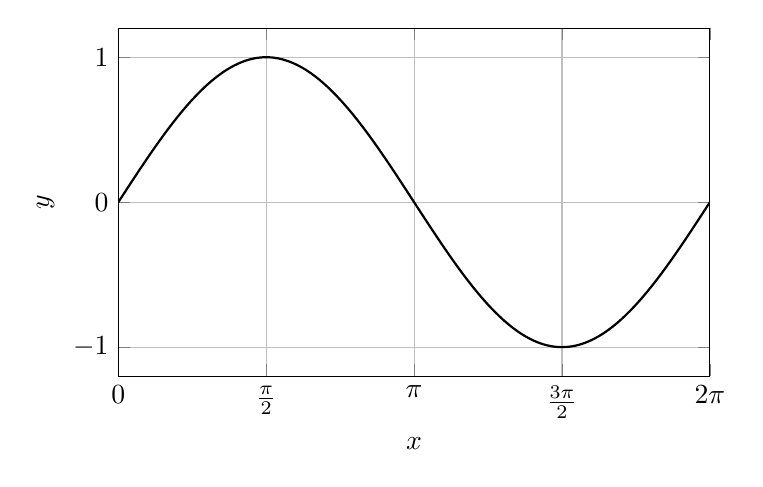
\begin{tikzpicture}
    \begin{axis}[
      width=0.75\textwidth,
      height=6cm,
      xlabel={$x$},
      ylabel={$y$},
      domain=0:6.28318,
      samples=200,
      grid=both,
      xmin=0, xmax=6.28318,
      ymin=-1.2, ymax=1.2,
      xtick={0,1.5708,3.1416,4.7124,6.2832},
      xticklabels={$0$, $\frac{\pi}{2}$, $\pi$, $\frac{3\pi}{2}$, $2\pi$},
    ]
      \addplot[thick] {sin(deg(x))};
    \end{axis}
  \end{tikzpicture}
  \caption{$y = \sin x$ grafikonja az $[0, 2\pi]$ intervallumon.}
  \label{fig:sin-plot-example}
\end{safemathfigure}
\newpage
\section{Matematikai ábrák kikapcsolása}

Ha a dolgozat egy vázlatosabb verzióját szeretnénk generálni, előfordulhat, hogy a matematikai ábrákat ideiglenesen el szeretnénk rejteni.  
Ezt megtehetjük a \texttt{showmathfigures} logikai kapcsolóval, amely a \texttt{szte-thesis.cls} fájlban van definiálva.  

\begin{codeblock}[caption={Matematikai ábrák kikapcsolása}]{TeX}
\setboolean{showmathfigures}{false}
\end{codeblock}

\section{UML diagramok (kikapcsolható ábrák)}

Ebben a részben néhány gyakori UML diagramtípust mutatunk be.
Minden példa \texttt{safefigure} környezetben van.
A példák forrása a \texttt{code/} mappában található.
A fejezetben az \verb|\inputcode| parancs importálja a forrást.
A PDF-ben az ábra a \verb|\input{...}| paranccsal kerül be.

\subsection{UML osztálydiagram (class diagram)}

\inputcode[UML class diagram forras]{TeX}{code/ch04-uml-class.tex}

\begin{safefigure}
	\centering
	\begin{tikzpicture}
  \umlclass[x=0,y=0]{User}
  {+id: int\\+name: string}
  {+login()\\+logout()}

  \umlclass[x=6,y=0]{Order}
  {+number: string\\+createdAt: date}
  {+total(): money}

  \umlclass[x=3,y=-3]{OrderItem}
  {+sku: string\\+qty: int}
  {}

  \umluniassoc[mult1=1,mult2=0..*]{User}{Order}
  \umlcompo[mult2=1..*]{Order}{OrderItem}
\end{tikzpicture}


	\caption{UML osztalydiagram pelda.}
	\label{fig:uml-class}
\end{safefigure}

\subsection{UML szekvenciadiagram (sequence diagram)}

\inputcode[UML sequence diagram forras]{TeX}{code/ch04-uml-sequence.tex}

\begin{safefigure}
	\centering
	\begin{sequencediagram}
  \newthread{u}{User}
  \newinst{c}{Controller}
  \newinst{s}{Service}
  \newinst{r}{Repo}

  \begin{call}{u}{createOrder()}{c}{orderId}
    \begin{call}{c}{validate()}{s}{ok}
    \end{call}
    \begin{call}{c}{save(order)}{r}{ok}
    \end{call}
  \end{call}
\end{sequencediagram}


	\caption{UML szekvenciadiagram pelda.}
	\label{fig:uml-sequence}
\end{safefigure}

\subsection{UML use case diagram}

\inputcode[UML use case diagram forras]{TeX}{code/ch04-uml-usecase.tex}

\begin{safefigure}
	\centering
	\begin{tikzpicture}
	\umlactor[x=0,y=0]{User}
	
	\begin{umlsystem}[x=5,y=0]{WebApp}
		\umlusecase[name=ucLogin,y=1]{Login}
		\umlusecase[name=ucPlaceOrder,y=-1]{PlaceOrder}
		\umlusecase[name=ucTrackOrder,y=-3]{TrackOrder}
	\end{umlsystem}
	
	\umlassoc{User}{ucLogin}
	\umlassoc{User}{ucPlaceOrder}
	\umlassoc{User}{ucTrackOrder}
\end{tikzpicture}

	\caption{UML use case diagram pelda.}
	\label{fig:uml-usecase}
\end{safefigure}

\subsection{Allapotgep diagram (state machine jellegu)}

\inputcode[Allapotgep diagram forras]{TeX}{code/ch04-uml-state.tex}

\begin{safefigure}
	\centering
	\begin{tikzpicture}[>=Stealth, node distance=3.2cm, on grid, auto]
  \node[state, initial] (new) {NEW};
  \node[state, right=of new] (paid) {PAID};
  \node[state, below=of paid] (shipped) {SHIPPED};
  \node[state, right=of shipped] (done) {DONE};
  \node[state, below=of new] (canceled) {CANCELED};

  \path[->]
    (new) edge node {pay} (paid)
    (paid) edge node {ship} (shipped)
    (shipped) edge node {deliver} (done)
    (new) edge node {cancel} (canceled)
    (paid) edge node {cancel} (canceled);
\end{tikzpicture}


	\caption{Allapotgep pelda (UML state machine jelleg).}
	\label{fig:uml-state}
\end{safefigure}



\chapter{Irodalomjegyzék és hivatkozások kezelése}

Ebben a fejezetben azt mutatjuk be, hogyan érdemes irodalomjegyzéket készíteni \texttt{biblatex} segítségével.  
Bemutatjuk, milyen hasznos könyvek és online források érhetők el.  
Megnézzük, hogyan néz ki egy tétel a \texttt{.bib} fájlban.  
Áttekintjük, milyen lépésekkel kell fordítani a dokumentumot.  

\section{Hasznos könyvek és online források}

A \LaTeX{} „alapműve” Leslie Lamport könyve, \emph{LaTeX: A Document Preparation System}~\cite{lamport1994}.  
Ez a könyv részletesen bemutatja a rendszer működését és a tipikus dokumentumok felépítését.  

Haladóbb használathoz hasznos \emph{The \LaTeX\ Companion} második kiadása~\cite{mittelbach2004}.  
Ez a könyv rengeteg gyakorlati példát ad többek között az irodalomjegyzék-kezelésre is.  

A \texttt{biblatex} csomagnak saját, részletes kézikönyve van~\cite{biblatexmanual}.  
Ez a dokumentáció elérhető a CTAN-on.  
Ez írja le a csomag fontos opcióit és a rendelkezésre álló stílusokat.  

Online bevezetőt ad például az Overleaf „Bibliography management with biblatex” című cikke~\cite{overleaf-biblatex}.  

\section{Mi van egy \texttt{.bib} tételben?}

Az irodalomjegyzék forrásai egy \texttt{.bib} fájlban tárolódnak.  
Minden forrás egy \emph{tétel} (entry), amelynek van típusa és mezői.  
A típus lehet például \texttt{@book}, \texttt{@article} vagy \texttt{@online}.  
A mezők jellemzően a szerző, cím, év és kiadó adatokat tartalmazzák.  

Nézzük meg példaként a Lamport-könyv bejegyzését~\cite{lamport1994}.  
Egy lehetséges \texttt{@book} tétel így néz ki a \texttt{references.bib} fájlban:  

\begin{codeblock}[caption={Egyszerű \texttt{@book} tétel a \texttt{.bib} fájlban}]{TeX}
@book{lamport1994,
  author    = {Leslie Lamport},
  title     = {LaTeX: A Document Preparation System},
  edition   = {2},
  publisher = {Addison-Wesley},
  year      = {1994},
  address   = {Reading, Massachusetts},
  isbn      = {978-0201529838},
}
\end{codeblock}

A mezők szerepe az alábbi.  

\begin{itemize}
  \item \verb|lamport1994| a tétel kulcsa. Ezt használjuk a szövegben a \verb|\cite{lamport1994}| parancsban.  
  \item Az \verb|author| mező a szerző nevét tartalmazza.  
  \item A \verb|title| mező a mű címét adja meg.  
  \item Az \verb|edition| mező a kiadás számát tartalmazza.  
  \item A \verb|publisher| mező a kiadó nevét tárolja.  
  \item A \verb|year| mező a megjelenés évét adja meg.  
  \item Az \verb|address| mező a kiadás helyét tartalmazza.  
  \item Az \verb|isbn| mező a könyv ISBN azonosítója.  
\end{itemize}

Más típusú tételek hasonló felépítésűek, csak a típus és néhány mező más.  
Például egy \texttt{@manual} vagy \texttt{@online} tétel esetén az \verb|url| és az \verb|urldate| mező is szerepelhet.  

\section{Hivatkozás a szövegben}

Ha a Lamport-tétel szerepel a \texttt{.bib} fájlban, akkor a szövegben hivatkozhatunk rá.  

\begin{itemize}
  \item \verb|\cite{lamport1994}| egyszerű hivatkozást hoz létre, például: „A \LaTeX{} rendszer részletes leírását lásd \verb|\cite{lamport1994}|.”  
  \item \verb|\cite{lamport1994,mittelbach2004}| egyszerre több forrásra hivatkozik.  
\end{itemize}

A konkrét megjelenési forma a \texttt{biblatex} stílusától függ.  
A jelen sablonban az \texttt{ieee} stílus van beállítva, ezért sorszámozott, szögletes zárójeles hivatkozásokat kapunk.  

\section{Fordítási lépések \texttt{biblatex} + \texttt{biber} használatakor}

A \texttt{biblatex} alapértelmezetten a \texttt{biber} programot használja a feldolgozáshoz.  
Ez eltér a régi \texttt{bibtex}-es munkafolyamattól.  

\begin{enumerate}
  \item A preambulumban szerepeljen az \verb|\addbibresource{references.bib}| sor.  
  \item Futtassuk a fordítást: \verb|pdflatex main|.  
  \item Ezután futtassuk a \verb|biber main| parancsot.  
  \item Végül futtassuk még kétszer a \verb|pdflatex main| parancsot.  
\end{enumerate}

Az irodalomjegyzék tényleges kiíratását a \verb|\printbibliography| parancs végzi, amely a \texttt{main.tex} végén található.  

	\printdeclaration
	
	\printbibliography
	
\end{document}
